\addcontentsline{toc}{chapter}{LAMPIRAN}
\titleformat{\section}{\normalfont\bfseries}{\thesection}{1em}{}
% Format judul untuk bagian lampiran
\chapter*{LAMPIRAN}

%\thispagestyle{plain} % Halaman pertama bab menggunakan gaya plain
\newappendix{Lampiran 1. Hasil deteksi tangan dengan MediaPipe}\label{lampiran 1}
%%multi figure 5-10 abjad
% \begin{figure}[H]
%   \centering
%   % \includegraphics[width=\textwidth, height = 10cm]{}
%   \label{}
% \end{figure}
\begin{figure}[H]
    \centering
    \begin{subfigure}{0.48\textwidth}
        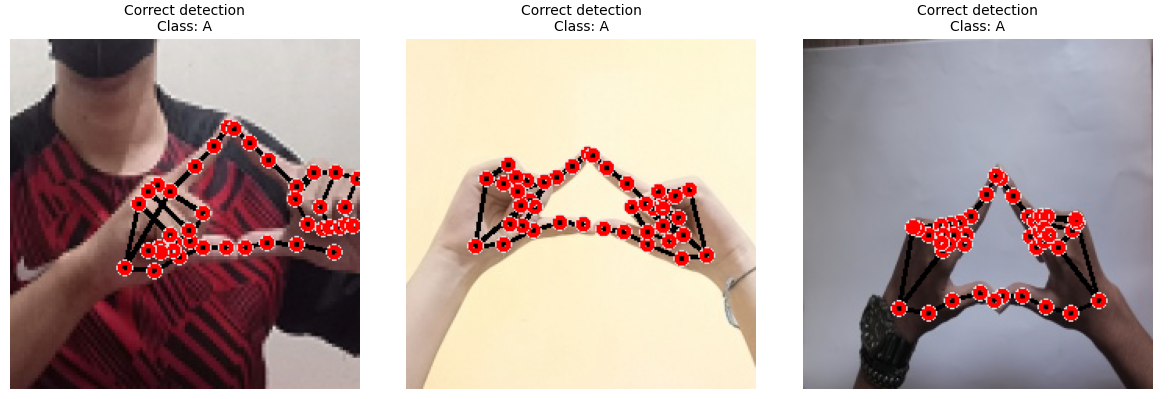
\includegraphics[width=\linewidth, height=3cm]{image/lampiran/kept_A.png} 
    \end{subfigure}
     \hfill
    \begin{subfigure}{0.48\textwidth}
        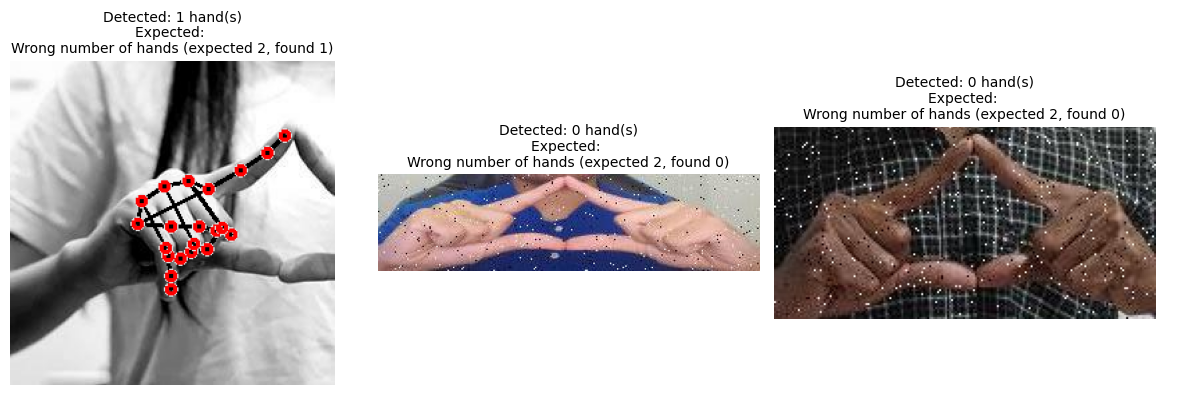
\includegraphics[width=\linewidth, height=3cm]{image/lampiran/failed_A.png} 
    \end{subfigure}

    \label{fig:hasil-deteksi-tangan}
\end{figure}


\newappendix{Lampiran 3. Diagram \textit{History} pelatihan model \textit{baseline}}
 \begin{figure}[H]
    \centering
    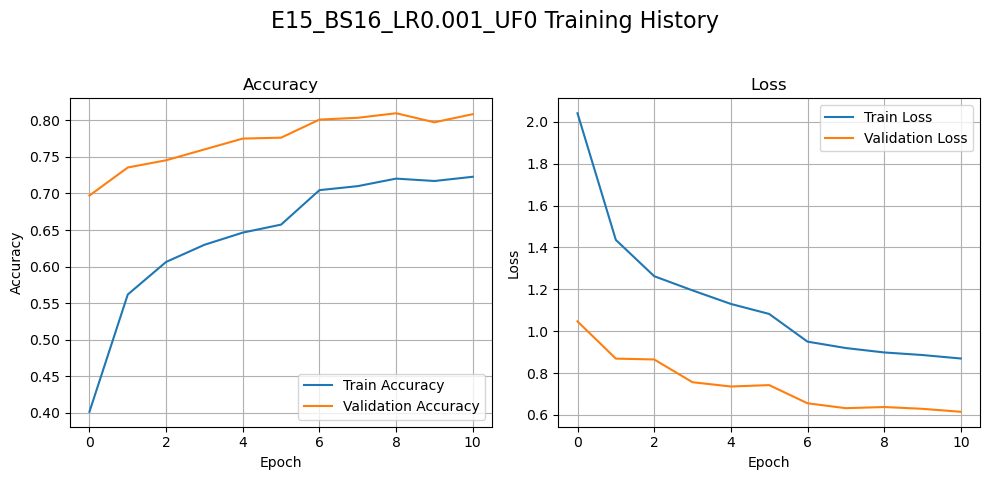
\includegraphics[width=\textwidth, height=5cm]{image/lampiran/mobilenetv2_baseline_history.png}
  \end{figure}

\newappendix{Lampiran 4. \textit{Classification Report} \textit{baseline}}
{\footnotesize
\begin{longtable}{|c|c|c|c|c|}
\hline
\textbf{Huruf} & \textit{\textbf{Precision}} & \textit{\textbf{Recall}} & \textit{\textbf{F1-score}} & \textit{\textbf{Support}} \\
\hline
\endfirsthead
\hline
\textbf{Huruf} & \textit{\textbf{Precision}} & \textit{\textbf{Recall}} & \textit{\textbf{F1-score}} & \textit{\textbf{Support}} \\
\hline
\endhead
A & 0.86 & 0.96 & 0.91 & 25 \\\hline
B & 0.76 & 0.90 & 0.83 & 29 \\\hline
C & 0.79 & 0.94 & 0.86 & 48 \\\hline
D & 0.69 & 0.47 & 0.56 & 19 \\\hline
A & 0.86 & 0.96 & 0.91 & 25 \\\hline
B & 0.76 & 0.90 & 0.83 & 29 \\\hline
C & 0.79 & 0.94 & 0.86 & 48 \\\hline
D & 0.69 & 0.47 & 0.56 & 19 \\\hline
A & 0.86 & 0.96 & 0.91 & 25 \\\hline
B & 0.76 & 0.90 & 0.83 & 29 \\\hline
C & 0.79 & 0.94 & 0.86 & 48 \\\hline
D & 0.69 & 0.47 & 0.56 & 19 \\\hline
\textit{\textbf{Accuracy}} &  &  & 0.82 & 820 \\ \hline
\textit{\textbf{Macro Avg}} & 0.80 & 0.79 & 0.79 & 820 \\ \hline
\textit{\textbf{Weighted Avg}} & 0.82 & 0.82 & 0.81 & 820 \\
\hline
\end{longtable}
}

% Please add the following required packages to your document preamble:
% \usepackage{longtable}
% Note: It may be necessary to compile the document several times to get a multi-page table to line up properly
% \begin{longtable}[c]{|l|l|l|l|l|l|l|l|}
%   \hline
%   \textit{\textbf{Dataset}} &
%     \textit{\textbf{Epochs}} &
%     \textit{\textbf{\begin{tabular}[c]{@{}l@{}}Batch \\ size\end{tabular}}} &
%     \textit{\textbf{\begin{tabular}[c]{@{}l@{}}Learning \\ rate\end{tabular}}} &
%     \textbf{Akurasi} &
%     \textbf{BLEU-1} &
%     \textbf{BLEU-2} &
%     \textbf{BLEU-3} \\ \hline
%   \endfirsthead
%   %
%   \endhead
%   %

%   \end{longtable}

\newappendix{Lampiran 5. Hasil pelatihan dengan BLIP untuk pertanyaan \textit{close ended}}

% Please add the following required packages to your document preamble:
% \usepackage{longtable}
% Note: It may be necessary to compile the document several times to get a multi-page table to line up properly
\begin{longtable}[c]{|l|l|l|l|l|l|l|l|}
    \hline
    \textit{\textbf{Dataset}} &
      \textit{\textbf{Epochs}} &
      \textit{\textbf{\begin{tabular}[c]{@{}l@{}}Batch \\ size\end{tabular}}} &
      \textit{\textbf{\begin{tabular}[c]{@{}l@{}}Learning \\ rate\end{tabular}}} &
      \textbf{Akurasi} &
      \textbf{BLEU-1} &
      \textbf{BLEU-2} &
      \textbf{BLEU-3} \\ \hline
    \endfirsthead
    %
    \endhead
    %
    PathVQA & 15 & 8  & $1 \times 10^{-5}$ & 83,44\% & 83,44 & 26,38 & 18,25 \\ \hline
    PathVQA & 15 & 8  & $5 \times 10^{-5}$ & 49,27\% & 49,27 & 15,58 & 10,78 \\ \hline
    PathVQA & 15 & 16 & $1 \times 10^{-5}$ & 72,38\% & 72,38 & 22,89 & 15,83 \\ \hline
    PathVQA & 15 & 16 & $5 \times 10^{-5}$ & 82,85\% & 82,85 & 26,20 & 18,13 \\ \hline
    PathVQA & 15 & 32 & $1 \times 10^{-5}$ & 64,24\% & 64,24 & 20,32 & 14,05 \\ \hline
    PathVQA & 15 & 32 & $5 \times 10^{-5}$ & 79,25\% & 79,25 & 25,06 & 17,34 \\ \hline
    PathVQA & 30 & 8  & $1 \times 10^{-5}$ & 77,15\% & 77,15 & 24,40 & 16,88 \\ \hline
    PathVQA & 30 & 8  & $5 \times 10^{-5}$ & 75,46\% & 75,46 & 23,86 & 16,51 \\ \hline
    PathVQA & 30 & 16 & $1 \times 10^{-5}$ & 74,43\% & 74,43 & 23,54 & 16,28 \\ \hline
    PathVQA & 30 & 16 & $5 \times 10^{-5}$ & 71,00\% & 71,00 & 22,45 & 15,53 \\ \hline
    PathVQA & 30 & 32 & $1 \times 10^{-5}$ & 76,11\% & 76,11 & 24,07 & 16,65 \\ \hline
    PathVQA & 30 & 32 & $5 \times 10^{-5}$ & 86,00\% & 86,00 & 27,20 & 18,82 \\ \hline
    PathVQA & 45 & 8  & $1 \times 10^{-5}$ & 76,02\% & 76,02 & 24,04 & 16,63 \\ \hline
    PathVQA & 45 & 8  & $5 \times 10^{-5}$ & 44,42\% & 44,42 & 14,05 & 9,72  \\ \hline
    PathVQA & 45 & 16 & $1 \times 10^{-5}$ & 77,33\% & 77,33 & 24,45 & 16,92 \\ \hline
    PathVQA & 45 & 16 & $5 \times 10^{-5}$ & 81,77\% & 81,77 & 25,86 & 17,89 \\ \hline
    PathVQA & 45 & 32 & $1 \times 10^{-5}$ & 76,56\% & 76,56 & 24,21 & 16,75 \\ \hline
    PathVQA & 45 & 32 & $5 \times 10^{-5}$ & 81,70\% & 81,70 & 25,83 & 17,87 \\ \hline
    VQA-RAD & 15 & 8  & $1 \times 10^{-5}$ & 61,54\% & 61,54 & 19,46 & 13,46 \\ \hline
    VQA-RAD & 15 & 8  & $5 \times 10^{-5}$ & 56,90\% & 56,90 & 17,99 & 12,45 \\ \hline
    VQA-RAD & 15 & 16 & $1 \times 10^{-5}$ & 0,84\%  & 0,84  & 0,27  & 0,18  \\ \hline
    VQA-RAD & 15 & 16 & $5 \times 10^{-5}$ & 51,24\% & 51,24 & 16,20 & 11,21 \\ \hline
    VQA-RAD & 15 & 32 & $1 \times 10^{-5}$ & 0,90\%  & 0,90  & 0,28  & 0,20  \\ \hline
    VQA-RAD & 15 & 32 & $5 \times 10^{-5}$ & 46,49\% & 46,49 & 14,70 & 10,17 \\ \hline
    VQA-RAD & 30 & 8  & $1 \times 10^{-5}$ & 22,94\% & 22,94 & 7,25  & 5,02  \\ \hline
    VQA-RAD & 30 & 8  & $5 \times 10^{-5}$ & 52,85\% & 52,85 & 16,71 & 11,56 \\ \hline
    VQA-RAD & 30 & 16 & $1 \times 10^{-5}$ & 9,35\%  & 9,35  & 2,96  & 2,04  \\ \hline
    VQA-RAD & 30 & 16 & $5 \times 10^{-5}$ & 45,00\% & 45,00 & 14,23 & 9,84  \\ \hline
    VQA-RAD & 30 & 32 & $1 \times 10^{-5}$ & 1,67\%  & 1,67  & 0,53  & 0,36  \\ \hline
    VQA-RAD & 30 & 32 & $5 \times 10^{-5}$ & 10,00\% & 10,00 & 3,16  & 2,19  \\ \hline
    VQA-RAD & 45 & 8  & $1 \times 10^{-5}$ & 34,17\% & 34,17 & 10,80 & 7,47  \\ \hline
    VQA-RAD & 45 & 8  & $5 \times 10^{-5}$ & 56,67\% & 56,67 & 17,92 & 12,40 \\ \hline
    VQA-RAD & 45 & 16 & $1 \times 10^{-5}$ & 12,50\% & 12,50 & 3,95  & 2,73  \\ \hline
    VQA-RAD & 45 & 16 & $5 \times 10^{-5}$ & 47,50\% & 47,50 & 15,02 & 10,39 \\ \hline
    VQA-RAD & 45 & 32 & $1 \times 10^{-5}$ & 3,33\%  & 3,33  & 1,05  & 0,73  \\ \hline
    VQA-RAD & 45 & 32 & $5 \times 10^{-5}$ & 51,67\% & 51,67 & 16,34 & 11,30 \\ \hline
    \end{longtable}

% Please add the following required packages to your document preamble:
% \usepackage{longtable}
% Note: It may be necessary to compile the document several times to get a multi-page table to line up properly
% Please add the following required packages to your document preamble:
% \usepackage{longtable}
% Note: It may be necessary to compile the document several times to get a multi-page table to line up properly
% Please add the following required packages to your document preamble:
% \usepackage{longtable}
% Note: It may be necessary to compile the document several times to get a multi-page table to line up properly
% \begin{longtable}[c]{|l|l|l|l|l|l|l|l|}
%     \hline
%     \textit{\textbf{Dataset}} &
%       \textit{\textbf{Epochs}} &
%       \textit{\textbf{\begin{tabular}[c]{@{}l@{}}Batch \\ size\end{tabular}}} &
%       \textit{\textbf{\begin{tabular}[c]{@{}l@{}}Learning \\ rate\end{tabular}}} &
%       \textbf{Akurasi} &
%       \textbf{BLEU-1} &
%       \textbf{BLEU-2} &
%       \textbf{BLEU-3} \\ \hline
%     \endfirsthead
%     %
%     \endhead
%     \end{longtable}

\begin{landscape}

\newappendix{Lampiran X. Tabel Lowongan Pekerjaan}

{\scriptsize
\begin{longtable}{|
    p{1.3cm}|  % Job ID
    p{2cm}|  % Title
    p{2cm}|  % Company
    p{1.5cm}|  % Location
    >{\raggedright\arraybackslash}p{2.5cm}|  % Link
    >{\raggedright\arraybackslash}p{4cm}|  % Job Description
    p{2cm}|    % Seniority
    p{1.5cm}|  % Employment
    p{2cm}|  % Function
    p{2cm}|  % Industry
|}
\hline
\textbf{Job ID} & 
\textbf{Title} & 
\textbf{Company} & 
\textbf{Location} & 
\textbf{Link} & 
\textbf{Job Description} & 
\textbf{Seniority} & 
\textbf{Employment} & 
\textbf{Function} & 
\textbf{Industry} \\
\hline
\endfirsthead

\hline
\textbf{Job ID} & 
\textbf{Title} & 
\textbf{Company} & 
\textbf{Location} & 
\textbf{Link} & 
\textbf{Job Description} & 
\textbf{Seniority} & 
\textbf{Employment} & 
\textbf{Function} & 
\textbf{Industry} \\
\hline
\endhead

4212612907 & 
ABAP Developer & 
PT Lion Super Indo & 
Jakarta, Indonesia & 
\href{https://id.linkedin.com/jobs/view/abap-developer-at-pt-lion-super-indo-4212612907}{ABAP Developer Lion} & 
Designs, develops, tests, debugs and implements SAP requirements based on functional and design documents. Requires Bachelor's in CS or related field, minimum 2 years as ABAP developer. Knowledge of SAP MM, SD, FI, CO. Optional SAP IS-Retail or FICO. Skills: ABAP, BADI, Smartforms, LSMW. Logical, customer-oriented, team player. & 
Mid-Senior level & 
Full-time & 
Information Technology & 
Retail \\
\hline

4210260823 & 
Graduate Development Program - Merger \& Acquisition - Jakarta & 
PT Asian Bulk Logistics & 
Jakarta, Indonesia & 
\href{https://id.linkedin.com/jobs/view/graduate-development-program-merger-acquisition-jakarta-at-pt-asian-bulk-logistics-4210260823}{Merger \& Acquisition} & 
12-month program with full-time opportunity. Aimed at fresh grads (Bachelor/Master) with max. 2 years experience. Jakarta-based. The company operates in logistics for mining and aims to become a global player in dry bulk sea cargo logistics. & 
Internship & 
Full-time & 
Business Development and Sales & 
Transportation, Logistics, Supply Chain and Storage \\
\hline

\end{longtable}
}

\end{landscape}


  \newappendix{Lampiran 6. Biodata Penulis}

  %\includepdf[pages=-]{tanda-tangan/biodata-signed.pdf} --> Jika sudah ada tanda tangan, komen code bawah dan uncomment code ini

  % space kebawah 1 spasi
  \bigskip
  \vspace{1sp}
  % teks dengan font 14 ke tengah
  \begin{center}
      \fontsize{14}{16}\selectfont
      \textup{\textbf{BIODATA}}
  \end{center}
  % space kebawah 2 spasi
  \vspace{2sp}

  \begin{tabbing}
    \hspace{2in} \= \hspace{2in} \kill
    1. Nama \> : XXXX XXXXX \\
    2. Tempat, tanggal lahir \> :  XXXXXXX, 00 Bulan 20XX \\
    3. Alamat \> : - \\
    4. Nama Ayah \> :  - \\
    5. Pekerjaan Ayah \> : Pekerjaan \\
    6. Nama Ibu \> : - \\
    7. Pekerjaan Ibu \> : Pekerjaan Ibu \\
    8. Alamat Orang Tua \> : Jl namajalan no XX , Banda Aceh \\
    9. Riwayat Pendidikan \> : 
  \end{tabbing}

  \begin{table}[H]
  \centering
  \resizebox{\textwidth}{!}{%
  \begin{tabular}{|c|c|c|c|c|}
  \hline
  \multicolumn{1}{|l|}{Jenjang} & \multicolumn{1}{l|}{Nama Sekolah} & \multicolumn{1}{l|}{Bidang Studi} & \multicolumn{1}{l|}{Tempat} & \multicolumn{1}{l|}{Tahun Ijazah} \\ \hline
  SD  & SD  Banda Aceh     & -   & Banda Aceh & 20XX \\ \hline
  SMP & SMP Banda Aceh & -   & Banda Aceh & 20XX \\ \hline
  SMA & SMA Banda Aceh & IPA & Banda Aceh & 20XX \\ \hline
  \end{tabular}%
  }
  \end{table}


  \begin{tabular}{p{7.5cm}l}
    &Banda Aceh, 00 Juli 20XX\\
    &\\
    &\\
    &\multirow{1.5}{7.5cm}{\underline{Nama Nama}} \\ 
    &NPM. XX081070100XX \\
  \end{tabular}

      